% documentclass
\documentclass[a4paper, 12pt]{article}
\usepackage[left= 3cm,right = 2cm, bottom = 4 cm]{geometry}
\usepackage[onehalfspacing]{setspace}
\usepackage[T1]{fontenc}
\usepackage[utf8]{inputenc}

% ============= Packages =============

% document information
%\usepackage[
%	pdftitle={Praxisarbeit},
%	pdfsubject={Mender.io Evaluation},
%	pdfauthor={Hannes Dürr},
%	pdfkeywords={},	
%	hidelinks,
%	backref=page
%]{hyperref}

% Basic Packages
\usepackage[ngerman]{babel}
\usepackage{graphicx, subfig}
\graphicspath{{images/}}
\usepackage{fancyhdr}
\usepackage{color}
\usepackage{listings}

% Dokumentinformationen
\usepackage[
	%Links nicht einrahmen
	hidelinks
]{hyperref}

\bibliographystyle{unsrt}

% Settings for ANSI-C-Code with frame and linebreak
\lstset{
	language=C,
	frame=single,
	breaklines=true,
}

% Package für extended lists
\usepackage{paralist}

% Package for units
%\usepackage{siunitx}

% Package for glossary
%\usepackage[acronym,automake]{glossaries}

% ============= header and footer =============
\pagestyle{fancy}
%
\lhead{}
\chead{}
\rhead{\slshape Hannes Dürr und Thomas Hollmann}
%%
\lfoot{}
\cfoot{\thepage}
\rfoot{}
%%
%\renewcommand{\headrulewidth}{0.4pt}
%\renewcommand{\footrulewidth}{0pt}

% ============= Dokumentbeginn =============

\begin{document}

\thispagestyle{empty} 

% ============== titel page ================
\begin{center}
\begin{tabular}{p{\textwidth}}


\begin{center}

\includegraphics[scale=0.5]{images/logo.png}
\end{center}


\\

\begin{center}
\LARGE{\textsc{Konzeption und Implementierung eines Schachcomputers von Grund auf}}
\end{center}

\\


\begin{center}
\large{Fakultät für Elektrotechnik, Feinwerktechnik und Informationstechnik\\
der Technischen Hochschule Nürnberg \\}
\end{center}

\\


\begin{center}
\large{Hannes Dürr and Thomas Hollmann} \\
\end{center}

\begin{center}
\large{September 2020}
\end{center}


\end{tabular}

\end{center}

\pagestyle{fancy}

\newpage

\tableofcontents

\newpage


\section{Einleitung}
Im Jahre 1948 veröffentliche Claude Shannon sein Paper \glqq{}Programming a Computer for Playing Chess\grqq{} und setzte damit den Startschuss für die Schachprogrammierung.
Nach 50 Jahren war es dann soweit und der erste Schachcomputer besiegte den amtierenden Schachweltmeister in einem Match mit 6 Partien und einem Endergebnis von 3,5 zu 2,5.
Der Schachcomputer namens \glqq{}Deep Blue\grqq{} basierte auf einem Minimax Algorithmus und berechnete 200 Millionen Stellungen pro Sekunde.
Heutige Schachengines finden mit nur 3 Millionen Stellungen pro Sekunde auf durchschnittlicher Heimcomputer-Hardware sogar noch besser Züge.\\
Ein Problem das heutige Engines allerdings haben ist, dass sie definitiv nicht anfängerfreundlich programmiert sind. Dies klingt erstmals nach einem sehr banalen Problem, allerdings schreckt dies junge motivierte Programmierer und Schach begeisterte ab und sorgt somit dafür, dass die Schachprogramming Community keinen sonderlich starken Zuwachs hat.
Diese Arbeit verfolgt das Ziel einer Einführung in das Thema Schachcomputer und ihre Programmierung zu geben. Es wird die Architektur einer Engine erläutert, die von Grund auf neu geschrieben wurde, mit dem Fokus auf einfachen, leicht zu verstehenden, aber trotzdem performanten Algorithmen.

\pagebreak
\section{Aufbau der Engine}

Das Ziel war es eine Schachengine von Grund auf zu programmieren, der Fokus lag hierbei auf einer einfachen, leicht zu verstehenden, aber trotzdem performanten Struktur.
Nachdem Thomas Hollmann aktiv im Schachverein ist und in der Regionalliga spielt, gab es die Möglichkeit Spielstärke zu analysieren und einzuschätzen. \\
Die Frage, die einen das Projekt hindurch begleitete, war:"wie bringt man das einer Schachengine bei ?".
Begonnen wurde mit dem Schachbrett, ein 8x8 Felder großes Brett, wobei sich die Farben der Felder horizontal wie auch vertikal abwechseln.
Da die Farbe der Felder bei der Zugfindung nicht relevant ist, wurde sie bei der Wahl der Datenstruktur nicht betrachtet.
Die anfängliche Idee war ein Array von 64 Integer-Variablen, womit jedes Feld durch eine Variable repräsentiert wird.
Nach etwas Recherche wurde das Array allerdings um 56 Plätze erweitert.\cite{10x12}\\
Dies repräsentiert ein 10x12 Feld, mit der Möglichkeit einen Rahmen aus \glqq{}-1\grqq{} um das eigentliche Spielfeld zu setzen.
Durch den Rahmen lässt sich  nun feststellen ob eine Figur durch einen Zug das Spielbrett verlässt und der Zug somit illegal wäre.
Nach einiger weiterer Recherche stößt man auch noch auf die Repräsentation durch ein Bitboard.
Hierbei wird nicht ein Feld dargestellt sondern jede Figur in einer 64 Bit großen Variable, was die Züge noch performanter macht.\cite{bitboard}\\
Da unser Fokus auf Übersichtlichkeit lag und wir auch schon zu fortgeschritten mit dem Projekt waren hatten wir uns allerdings dagegen entschieden und sind bei der Brettdarstellung durch ein Array mit 120 Integer Werten geblieben.
Bei dieser Variante wurde den Figuren je ein Zahlenwert zugeordnet, wobei sich die Zahlenwerte der weißen und schwarzen Figuren jeweils um 10 unterscheiden, was die weitere Programmierung deutlich erleichterte. Im Folgenden ist das fertige Array \glqq{}board\grqq{} mit den Figuren in der Startposition zu sehen.\\

\pagebreak

\begin{lstlisting}

int board[120] = {-1,-1,-1,-1,-1,-1,-1,-1,-1,-1,
                  -1,-1,-1,-1,-1,-1,-1,-1,-1,-1,
                  -1,14,12,13,15,16,13,12,14,-1,
                  -1,11,11,11,11,11,11,11,11,-1,
                  -1,00,00,00,00,00,00,00,00,-1,
                  -1,00,00,00,00,00,00,00,00,-1,
                  -1,00,00,00,00,00,00,00,00,-1,
                  -1,00,00,00,00,00,00,00,00,-1,
                  -1,01,01,01,01,01,01,01,01,-1,
                  -1,04,02,03,05,06,03,02,04,-1,
                  -1,-1,-1,-1,-1,-1,-1,-1,-1,-1,
                  -1,-1,-1,-1,-1,-1,-1,-1,-1,-1,};
\end{lstlisting}

Um nun die Figuren bewegen zu lassen und den bestmöglichen Zug zu finden, wurde der Movegenerator() erstellt.
Dieser iteriert über das board und führt, je nach dem welche Farbe am Zug ist,  bei jeder zugehörigen Figur alle möglichen Züge aus.
Die Basiszüge lassen sich recht einfach ausführen und wurden über ein Richtungs-Array implementiert, welches die möglichen Bewegungsrichtungen einer Figur enthält, sowie die Anzahl der möglichen Bewegungsrichtungen.
Im Folgenden ist das Richtungs-Array des Springers zu sehen, mit acht möglichen Richtungen.

\begin{lstlisting}
int dir_Kn[9]={8,12,-12,21,-21,8,-8,19,-19};
\end{lstlisting}

Findet der Movegenerator beim iterieren nun den weißen Springer, so werden die 8 möglichen Endfelder überprüft ob das Feld leer ist, illegal ist oder sich eine gegnerische Figur auf dem Feld befindet.

\begin{lstlisting}
if(board[Endfeld] == 0 || board[Endfeld] > 10)
\end{lstlisting}

\newpage

Eine Besonderheit kommt bei den Figuren Turm, Dame und Läufer hinzu, da sich diese Figuren in eine Richtung beliebig viele Felder bewegen können, solange die Felder frei sind.
Dies wurde über eine While schleife gelöst, die solange iteriert, bis ein illegales oder besetztes Feld erreicht wurde.
Wenn z.B. nach drei Iterationen festgestellt wird, dass der nächste Zug eine gegnerische Figur schlagen könnte, so wird die Figur geschlagen und dann die While-Schleife unterbrochen.

\begin{lstlisting}
while(board[neues_Feld] == 0 || board[neues_Feld] > 10) {
    /* Figur schlagen */
    if (board[neues Feld] > 10) {
        ...
        break
    }
    ...
    /* ein Feld weiter ziehen*/
    neues_Feld += dir_R[y];
}
\end{lstlisting}

Bei der Implementierung der Figuren sind zwei Figuren herausgestochen, welche nochmals gesondert betrachtet werden mussten.\\


Der Bauer mit seinen Regeln:
\begin{compactenum}
\item{Im normalen Spielverlauf darf er ein Feld nach vorne ziehen, soweit dies leer ist.}
\item{Der Bauer darf gegnerische Figuren diagonal schlagen.}
\item{Ist der Bauer noch auf seinem Anfangsfeld, darf er entweder 1 oder 2 Felder nach vorne ziehen, vorausgesetzt, diese sind leer.}
\item{Umwandlung: ist der Bauer auf der gegenüberliegenden Seite angekommen, so darf sich der Spieler aussuchen welche Figur man anstatt des Bauern auf diesem Feld haben möchte.
Gewählt werden darf zwischen den Figuren Dame, Turm, Läufer oder Springer.}

\newpage

\item{En Passant: Vorausgesetzt ist eine vergleichbare Situation: Zieht der weiße Spieler seinen Bauer von a2 auf a4, so hat der schwarze Spieler für exakt einen Zug die Möglichkeit diesen weißen Bauern mit seinem Bauern auf b4 en passant zu schlagen.\cite{enpassant}}
\end{compactenum}

\begin{center}
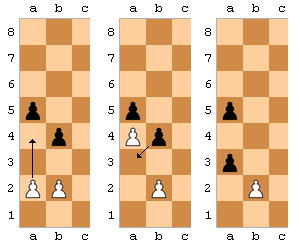
\includegraphics[scale=0.9]{images/enpassant.png}
\captionof{figure}{En passant Zug - Beispiel}
\end{center}

Die Schwierigkeit lag hier vor allem bei der Regel 5, da der Zug zum einen aus dem 2-Feld-Zugmuster raus fällt und hierbei 3 Felder geändert werden müssen und zum anderen Vergangenheitswerte benötigt werden, um festzustellen ob der schwarze Bauer einen Zug zuvor sich genau zwei Felder nach vorne bewegt hat.
Gelöst wurde die Problematik durch eine enpassant-Feld Variable, welches immer dann gesetzt wird wenn sich ein Bauer, egal von welcher Farbe aus der Grundreihe heraus zwei Felder nach vorne bewegt.
Der enpassant-Feld Variable wird dann das Feld zugewiesen, auf dem der Bauer nach dem Zug steht.
Ein Zug später fragt nun der Gegner ab ob das enpassant-Feld direkt neben einem seiner Bauern ist, ist dies der Fall so hat er die Möglichkeit den Bauern enpassant zu schlagen. Durch die Übergabe des enpassant-Feldes wird zusätzlich sichergestellt, dass der en passant Zug auch nur im darauf folgenden Zug möglich ist.

\begin{lstlisting}
if( (enpassant_square - square) == 1 ||
    (enpassant_square - square) == -1 ){
    /* move enpassant*/
    ...
}
\end{lstlisting}


Die zweite Figur die heraus gestochen ist, ist der König wegen der langen und kurzen Rochade.
Die Voraussetzungen für die Rochaden sind:\\


\begin{compactenum}
\item{Der König muss auf seinem Grundfeld stehen und darf bis dato noch nicht gezogen sein.}
\item{Der jeweilige Turm muss auf seinem Grundfeld stehen und darf bis dato noch nicht gezogen sein.}
\item{Die Felder zwischen König und jeweiligem Turm müssen frei sein.}
\item{Keines der 3 Felder auf denen der König sich während der Rochade bewegt darf von einer gegnerischen Figur angegriffen sein.}
\end{compactenum}

Die Regeln 1 und 2 führen zu dauerhaftem Rochade-Verlust, was über das gesamte Spiel hinweg vermerkt sein muss.
Hierfür wurden 4 globale Variablen angelegt, da sowohl der Movegenerator, als auch der Spieler darauf zugreifen muss.\\
Die Regel 3 und 4 verbieten die Rochade nur in diesem Moment. 

Der Movegenerator sollte nun alle möglichen Züge finden, ob dies tatsächlich der Fall ist lässt sich grob über die Shannon Nummer überprüfen\cite[Absatz: Shannon's calculation]{shannon_number}. Bei einer Rechentiefe von 5, sprich 5 halb-Zügen, berechnet die Engine 4.861.862 Stellungen. Shannon berechnet für diese Tiefe 4.865.609 Stellungen. Die Abweichung von ungefähr 4.000 Stellungen lässt sich dadurch erklären, dass Shannon bei seiner Berechnung einige legale Züge unterschlägt und andere illegale Züge mitberechnet.
Insgesamt ist das Ergebnis akzeptabel.
Die gefunden Züge müssen nun allerdings noch ausgeführt werden.
Hierfür kommt die changepos-Funktion ins Spiel, sie bekommt die Start- und Endposition der derzeitigen Figur gegeben, einen Zeiger auf eine Variable zum Merken der geschlagenen Figur und einen Zeiger auf das board.
\newpage


\begin{lstlisting}
void change_pos(int board[], int new_pos, int old_pos, int *copy_piece)
{
    /* save the piece to capture (on the new pos) so it can be returned */
    *copy_piece = board[new_pos];
    /* move the piece from the old position to the new position */
    board[new_pos] = board[old_pos];
    /* now the old position is empty */
    board[old_pos] = 0;
}
\end{lstlisting}

Nun wurden zwar alle möglichen Züge gefunden und ausgeführt, um aber herauszufinden welcher dieser Züge der Beste ist, ist es notwendig noch weiter in die Zukunft zu schauen und herauszufinden wie der Gegner auf den Zug antworten könnte.
Um dies zu erreichen wurde eine Tiefensuche implementiert. Die Movegenerator-Funktion ruft sich hierbei immer dann rekursiv selbst auf, wenn sie einen möglichen Zug gefunden hat.


\begin{lstlisting}
int move_gen( int board[], int depth, bool black_or_white, int enpassant_square, bool long_castle_w, bool long_castle_b, bool short_castle_w, bool short_castle_b )
\end{lstlisting}

Dieser Algorithmus erzeugt einen Baum, welcher sehr anschaulich ist.
Zu Beginn der Movegenerator-Funktion wird die Tiefe abgefragt, um nicht unendlich lange zu suchen.

\begin{lstlisting}
if ( depth == 0 ) {
    return evaluation(board);
}
\end{lstlisting}

Wird die gewünschte Tiefe erreicht, so wird die aktuelle Stellung an eine Evaluations-Funktion übergeben, welche die Qualität der Stellung als Zahl zurück gibt.
Die Evaluation der Stellung ist sehr simpel gehalten und betrachtet nur zwei Kriterien, die Anzahl an vorhandenem Material(Schachfiguren auf dem Brett) und die Kontrolle der mittleren Felder. 
Für die Überprüfung von vorhandenem Material wurde jedem Figuren-Typ eine Qualitätszahl zugeordnet, wobei die weißen Figuren positive, die Schwarzen negative Werte erhalten haben.

\begin{table}[h!]
\centering
\begin{tabular}{|| c | c ||} 
 \hline
 Figur & Wert \\
 \hline\hline
 Bauer & +-100  \\ 
 Springer & +-280  \\
 Läufer & +-300  \\
 Turm & +-500  \\
 Dame & +-900  \\
 König & +-100000  \\
 \hline
\end{tabular}
\caption{Die Evaluationswerte der Figuren}
\label{evaluation}
\end{table}

Nun iteriert die Funktion über das Brett, summiert die Qualitätszahl aller gefundenen Figuren zusammen und gibt die Summe als Rückgabewert zurück. Ist die Summe 0 so ist die Anzahl von vorhandenem Material für beide Seiten gleich.\\
Ein weiteres Evaluationskriterium ist die Kontrolle der mittleren Felder.
Hierfür werden die mittleren Felder d4 d5 e4 e5 abgefragt. Pro weißer Figur wird der Rückgabewert um 10 Punkte erhöht und pro schwarzer Figur um 10 Punkte verringert.\\
Bei Recherchen stößt man auf zahlreiche weitere Evaluationsmöglichkeiten, welche sich Modular hinzufügen lassen.\\

Nachdem die Stellung evaluiert wurde, wird der Zug, mit Hilfe der changeposback-Funktion, wieder rückgängig gemacht.
Diese verhält sich konträr zur changepos-Funktion.
Um nun wirklich durch und durch mit dem besten Zug für die jeweilige Farbe zu rechnen, wurde der MiniMax Algorithmus in der Movegenerator-Funktion angewandt.

\begin{center}
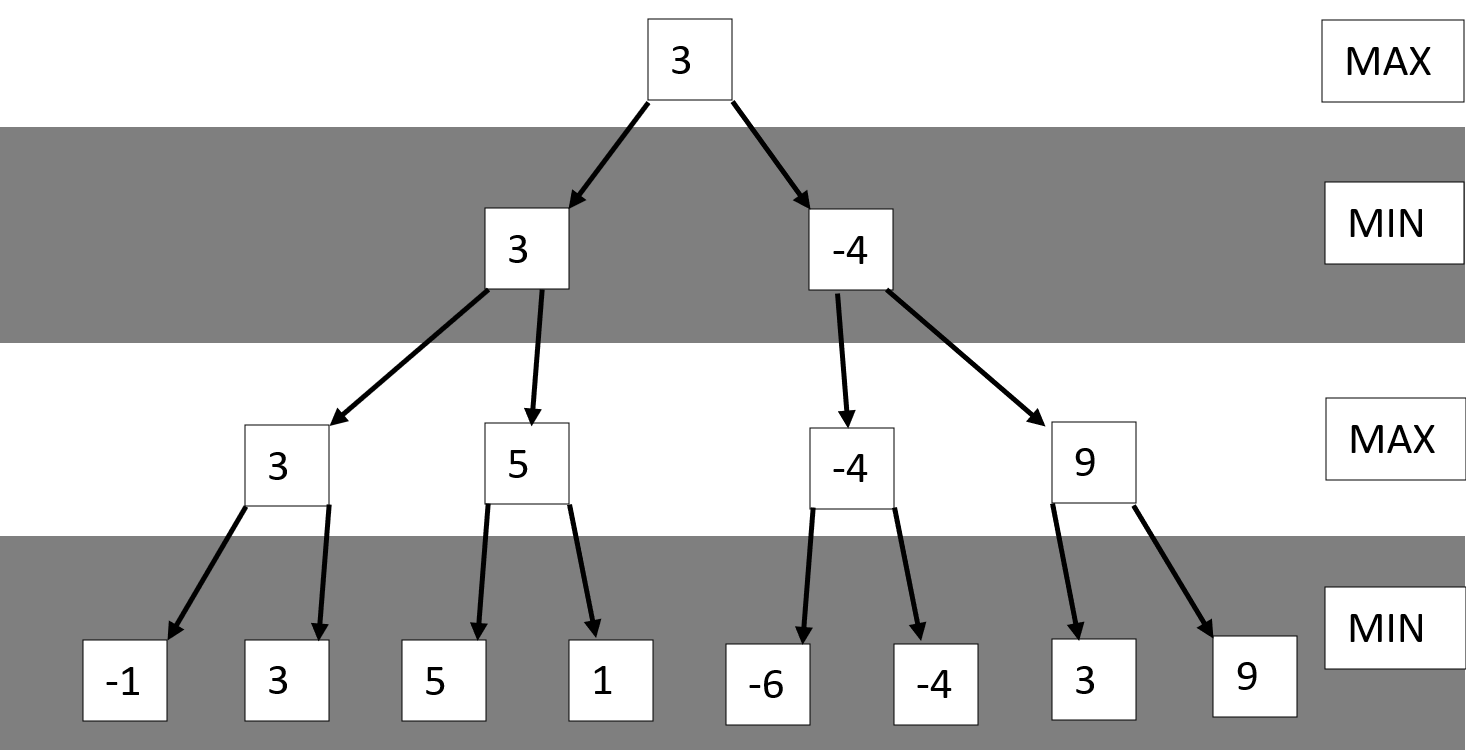
\includegraphics[scale=0.3]{images/minimax.png}
\captionof{figure}{Minimax Beispiel}
\end{center}

Hierbei wird, wie schon erwähnt und im Bild zu sehen, ein Baum aufgebaut. Es sei erwähnt, dass hier der einfachheitshalber ein Binärerbaum gezeigt wird, in einem normalen Spiel ist die Anzahl der Äste aber deutlich größer. An den untersten Stellen im Baum steht der Rückgabewert der Evaluationsfunktion. 
Der Algorithmus sieht nun vor, nach und nach die Blätter(äußersten/untersten Knoten) miteinander zu vergleichen. 
In dem Beispiel wird ein Zug für Weiß gesucht. Weiß ist der maximierende Spieler, sprich von allen verglichenen Blättern schafft es nur die größte Zahl eine Ebene weiter nach oben in den nächst höheren Knoten.\\


Dieser Vergleich wurde wie folgt implementiert:

\begin{lstlisting}
eval = move_gen(board, depth-1, false, false, long_castle_w, long_castle_b, short_castle_w, short_castle_b);
max = (eval > max ? eval : max);
...
...
return max;
\end{lstlisting}
Gleiches gilt auch für den schwarzen Spieler, wobei hier nach dem minimalen Evaluationswert gesucht wird.
Durch den Algorithmus stellt man nun fest welche Zugkombination für beide Seiten die Beste ist, allerdings gilt es dann noch den besten Zug zu extrahieren.
Hierzu wird abgefragt, ob die Funktion sich in der ersten Tiefe befindet, also an einem der zweit-obersten Knoten und ob der derzeitige Evaluationswert der Beste bisher ist.
Ist dies der Fall so weiß man, dass es sich um den derzeit besten Zug handeln muss.
Dieser wird deshalb abgespeichert und zwar in der globalen Struktur \glqq{}best\_move\grqq{}, damit der Zug später fest auf das Board geschrieben werden kann.
Des weiteren beinhaltet die Struktur eine Variable zur Anzeige, ob es sich um einen Spezialzug handelt(Rochade, Umwandlung, enpassant), da hier das eigentliche 2-Feld-Zugmuster nicht gilt.

\begin{lstlisting}
if((depth == MAXDEPTH) && (eval == max)){
    best_move->start_pos = square;
    best_move->end_pos = square+dir_wP[1];
    best_move->special = 0;
}
\end{lstlisting}

\pagebreak

Damit man nun wirklich gegen die Schachengine spielen kann, benötigt es noch ein User-Interface mit Zugeingabe, sowie eine Überprüfungen der Züge.
Für das User-Interface wurde die ncurses Library verwendet. Mit dieser ist eine zeichenorientierte Darstellung des Spiels im Terminal möglich.

\begin{center}
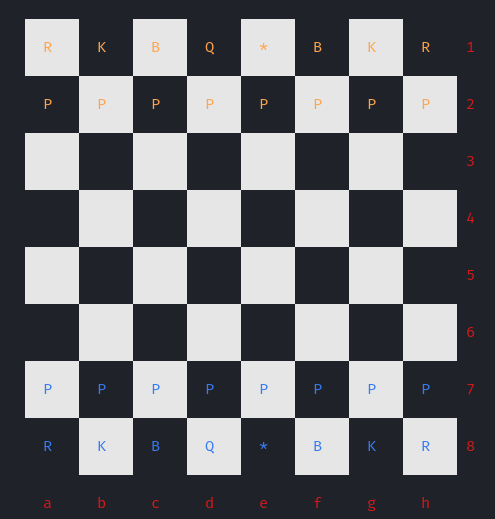
\includegraphics[scale=0.7]{images/ncurses_board.png}
\label{ncurses_board}
\captionof{figure}{Schachbrett Darstellung mit ncurses}
\end{center}

Die Zugeingabe fragt zuerst ab, ob es sich bei dem Zug um einen Spezialzug handelt. Danach wird das Startfeld und Endfeld des Zuges angegeben und der Zug auf dem Brett ausgeführt. Im Anschluss wird die Engine aufgerufen und gibt ihren besten Zug an. Auch dieser wird ausgeführt und das Prozedere wiederholt sich.\\
Bei jedem Zug wird zusätzlich noch überprüft, ob alle globalen Schachregeln eingehalten werden. Dazu zählen:

\begin{compactenum}
\item{Schachmatt: Spieler A hat keine Möglichkeit mehr zu verhindern, dass Spieler B den König von Spieler A im nächsten Zug schlagen kann.
Um dies zu überprüfen kann die Schachengine verwendet werden.
Sie überprüft mit Rechentiefe 2, ob nach jedem möglichen 1. Zug der 2. Zug den König schlagen kann, ist dies der Fall ist es Schachmatt und die Partie ist beendet.}
\item{Patt: Spieler A hat keine Möglichkeit mehr zu ziehen, ohne dass Spieler B den König von Spieler A im nächsten Zug schlagen kann. Gleichzeitig steht der König von Spieler A nicht im Schach.\\
Auch hierfür kann die Schachengine verwendet werden. Sie überprüft im Fall von Schachmatt, ob es nicht Patt ist, indem mit Rechentiefe 1 und umgedrehter Farbe geprüft wird, ob der König geschlagen werden kann. Kann er nicht geschlagen werden so ist es Patt und das Spiel endet Remis.}
\item{Zu wenig Material: Ist es mit den Figuren auf dem Brett nicht mehr möglich Schachmatt zu setzen, endet das Spiel mit einem Remis. Das ist der Fall, wenn weder Bauern, Türme noch Damen am Brett sind und auch weniger als Springer und Läufer auf am Brett stehen.
Gelöst wurde dies durch eine Funktion die über das board Iteriert und überprüft welche Figuren darauf stehen, sind es zu wenige endet das Spiel Remis.}
\item{50 Zug Regel: Werden 50 Weiße und 50 Schwarze Züge lang keine Figur geschlagen oder Bauern gezogen, so endet das Spiel in einem Remis.
Hierfür wird nach jedem Zug überprüft ob die genannte Bedingung erfüllt ist, ist dies der Fall, so wird der Zähler der move\_rule zurück gesetzt. Zusätzlich wird nach jedem Zug der Zähler inkrementiert. Wenn der Zähler die 100 Züge überschreitet, so wird das Spiel beendet.
\begin{lstlisting}
/* make_move()*/
if(board[end_pos] > 0 || board[start_pos] == 1 || board[start_pos] == 11)
	*move_rule = 0;

/* rule_50_move() */
move_rule++;
if(move_rule>100){
	game=0;
\end{lstlisting}
}

\end{compactenum}

\pagebreak

\section{Auswertung}
Die Performance eines Schachcomputers lässt sich technisch gesehen nur schwer messen. Zwar könnte man die Anzahl der berechneten Stellungen pro Sekunde vergleichen, wirklich aussagekräftig ist dies allerdings nicht, da  durch Pruning Algorithmen die Anzahl der zu berechnenden Stellungen deutlich abnimmt\cite[Absatz: savings]{alphabeta}.
Viel besser ist der Vergleich von Schachcomputerzügen bei verschiedenen Stellungen mit den Vorgeschlagenen Zügen einer professionellen Engine.
Hierbei wurde die Open-source Engine Stockfish(Version 11) zur Hilfe genommen.
Verglichen wurde eine Stellung aus der Spielmitte und zwei Stellung aus dem Endspiel.\\
Stellungen aus dem Spielanfang wurden nicht verglichen, da Professionelle Engines entweder mit einer Eröffnungsbibliothek arbeiten oder spezielle Implementierungen für den Spielanfang beinhalten und die hier beschriebene Engine schlicht und ergreifend keine wirklich vernünftigen Züge ausführt.\\

Stellung 1:
Zu sehen ist eine Position aus der Spielmitte. Stockfish wertet die Position als ausgeglichen (-0,1). Weiß ist am Zug.
\begin{center}
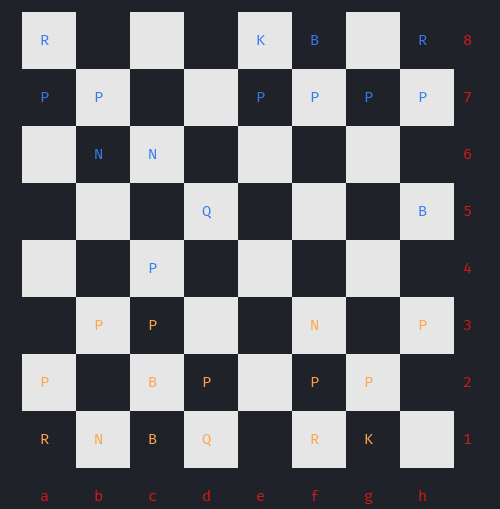
\includegraphics[scale=0.63]{images/st_2_1.png}
\label{ncurses_board}
\captionof{figure}{Ausgeglichene Stellung aus der Spielmitte}
\end{center}
Stockfish sieht den besten Zug für weiß in b3 c4. Spielt man diesen Zug, so antwortet unsere Engine mit einem Angriff der Dame d5 c4, was laut Stockfish zwar nicht der beste Zug ist, sondern b6 c4, aber trotzdem die Stellung sehr ausgeglichen lässt und Weiß dazu verpflichtet ihren Turm auf f1 zu verteidigen.
\begin{center}
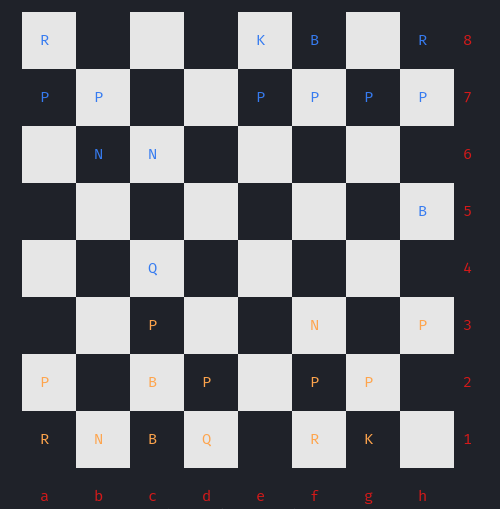
\includegraphics[scale=0.63]{images/st_2_2.png}
\label{ncurses_board}
\captionof{figure}{Antwort der Engine mit Dame d5 c4}
\end{center}

Stellung 2:
Zu sehen ist eine Endspiel Position in der schwarz mit König und zwei Türmen gegen den weißen König spielt. Weiß ist am Zug.
\begin{center}
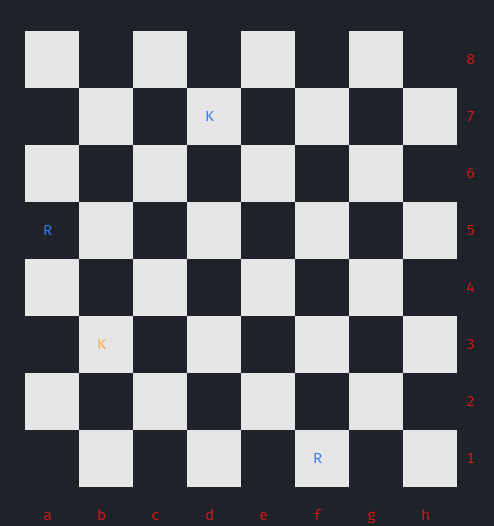
\includegraphics[scale=0.63]{images/st_1_1.png}
\label{ncurses_board}
\captionof{figure}{Endspiel mit König und zwei Türmen gegen König}
\end{center}
Stockfish sieht den besten Zug für Weiß in b3 b4. Spielt man diesen Zug, so antwortet unsere Engine mit einer Verteidigung des Turms durch f1 f5, was zwar erfolgreich verteidigt, aber leider Geschwindigkeit aus Stellung nimmt, wodurch es mehr Züge bis zum Schachmatt benötigt.
Im weiteren Spielverlauf verteidigt der Schachcomputer zwar erfolgreich seine Figuren aber schafft es nicht Schachmatt zusetzen.
Begründen lässt sich das zum einen durch die eingestellte Rechentiefe von 6 Zügen und zum anderen durch die noch fehlenden Evaluationseigenschaften.
\begin{center}
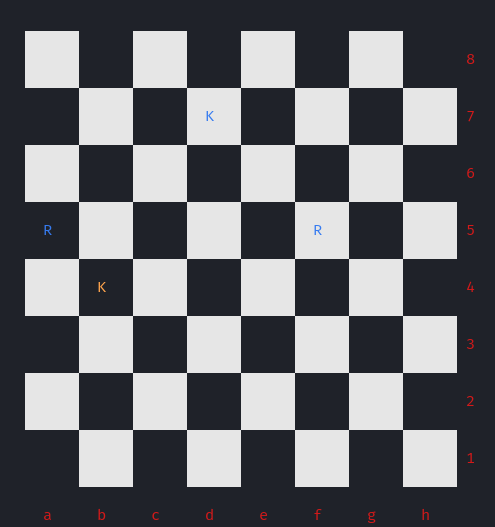
\includegraphics[scale=0.63]{images/st_1_2.png}
\label{ncurses_board}
\captionof{figure}{Antwort der Engine mit Turm f1 f5}
\end{center}

Abschließend lässt sich sagen, dass die Engine zwar sicherlich keinen Weltmeister schlägt und auch gegen Spieler mit etwas Erfahrung und Wissen über das Spiel wenig Chancen hat, aber trotzdem im Grunde Regel konforme Züge ausführt und ihren Gegner ab und an in die Bredouille führen kann.
Die nächsten Verbesserungsmaßnahmen wären die Implementierung eines Pruning Algorithmus, sowie die Erweiterung der Evaluationsfunktion.

\clearpage

\newpage

\sloppy

\bibliography{Literatur}

\end{document}
